\subsection{PROOF OF LEMMA 1}

Let \(\mathrm{E}_{s,s'}^*\) be the dual of the plane \(\mathrm{E}_{s,s'} = \mathbf{Re}_s\oplus \mathbf{Re}_{s'}\) (no. 2). The transpose of the injection \(\mathrm{E}_{s,s'}\to \mathrm{E}\) is a surjection

\[
p: \mathrm{E} ^ {*} \to \mathrm{E} _ {s, s ^ {\prime}} ^ {*}
\]

that commutes with the action of the group \(W_{s,s'}\) . It is clear that \(A_{s}\) , \(A_{s'}\) and \(A_{s} \cap A_{s'}\) are the inverse images under p of corresponding subsets of \(E_{s,s'}^{*}\) (considered as the space of the contragredient representation of the Coxeter group \(W_{s,s'}\) ). Moreover, since the length of an element of \(W_{s,s'}\) is the same with respect to \(\{s,s'\}\) and with respect to S (Chap. IV, §1, no. 8), we are reduced finally to the case where \(S = \{s,s'\}\) ; if \(m = m(s,s')\) , the group W is then a dihedral group of order 2m.

We now distinguish two cases:

\begin{enumerate}
\def\labelenumi{\alph{enumi})}
\tightlist
\item
  \(m = +\infty\) .
\end{enumerate}

Let \((\varepsilon, \varepsilon')\) be the dual basis of \((e_s, e_{s'})\) . Then

\[
s. \varepsilon = - \varepsilon + 2 \varepsilon^ {\prime}, s ^ {\prime}. \varepsilon = \varepsilon ,
\]

\[
s. \varepsilon^ {\prime} = \varepsilon^ {\prime}, s ^ {\prime}. \varepsilon^ {\prime} = 2 \varepsilon - \varepsilon^ {\prime}.
\]

Let D be the affine line of \(E^{*}\) containing \(\varepsilon\) and \(\varepsilon'\) ; the formulas above show that D is stable under s and \(s'\) and that the restriction of s (resp. \(s'\) ) to D is the reflection with respect to the point \(\varepsilon'\) (resp. \(\varepsilon\) ). Let

\[
\theta : \mathbf {R} \to \mathrm{D}
\]

be the affine bijection \(t \mapsto \theta(t) = t\varepsilon + (1 - t)\varepsilon'\) . Let \(I_n\) be the image under \(\theta\) of the open interval \(]n, n + 1[\) , and let \(C_n\) be the union of the \(\lambda I_n\) for \(\lambda > 0\) . Then \(C_0 = C\) ; moreover, by the Remark of §2, no. 4, applied to the affine space D, the \(I_n\) are permuted simply-transitively by W; hence so are the \(C_n\) . If \(v \in W\) , \(v(C)\) is equal to one of the \(C_n\) , hence is contained in \(A_s\) if \(n \geqslant 0\) and in \(s(A_s)\) if \(n < 0\) . In the second case, \(I_0\) and \(I_n\) are on opposite sides of the point \(\varepsilon'\) ; hence \(l(sv) = l(v) - 1\) (loc. cit.).

\begin{enumerate}
\def\labelenumi{\alph{enumi})}
\setcounter{enumi}{1}
\tightlist
\item
  m is finite.
\end{enumerate}

The form \(B_{M}\) is then non-degenerate (no. 2) so we can identify \(E^{*}\) with E. We have seen that E can be oriented so that the angle between the half-lines \(R_{+}e_{s}\) and \(R_{+}e_{s'}\) is equal to \(\pi - \frac{\pi}{m}\) . Let D (resp. \(D'\) ) be the half-line obtained from \(R_{+}e_{s}\) (resp. \(R_{+}e_{s'}\) ) by a rotation of \(\pi/2\) (resp. \(-\pi/2\) ), cf.~Fig. 2. The chamber C is the set of \(x \in E\) whose scalar product with \(e_{s}\) and \(e_{s'}\) is \textgreater0; this is the open angular sector with origin \(D'\) and extremity D. By the Remark of §2, no. 5, every element v of W transforms C into an angular sector that is on the same side of D as C (i.e.~is contained in \(A_{s}\) ) or on the opposite side (i.e.~contained in \(s(A_{s})\) ), and in the latter case

\[
l (s v) = l (v) - 1,
\]

which completes the proof of the lemma.

\pandocbounded{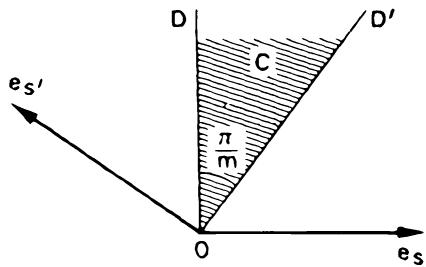
\includegraphics[keepaspectratio]{images/part001_dfbe6528.jpg}}\\
Fig. 2

